\section{The off-shell window}\label{sec:13.6}

At $|\vect{q}| = \SI{1.0}{keV}$ along the valley axis the cheapest zero-phonon pair of silicon costs \SI{1.77}{eV}, and the phonon-assisted structure factor of \cref{sec:13.3} was written for energies below it. Two kinds of denominators in the amplitude \cref{eq:13.2-M} can become small. Those of path A with an empty band and of path C with a filled band are the distances of virtual zero-phonon pairs from the energy shell, and they vanish as $\omega$ reaches $E_{\mathrm{min}}(\vect{q})$. The intraband terms, path A with $p = c$ and path B with $p = v$, have denominators of order $|\vect{Q}|$ and vanish as the phonon becomes a soft acoustic one, while the interband vertices of that phonon grow as $|\vect{Q}|^{-1/2}$. The soft acoustic phonon produces no divergence: translation invariance fixes its amplitude, and inside the window it is never on the energy shell. The vanishing zero-phonon detunings, however, set the boundary of the region in which the phonon-assisted rate exists as a quantity of its own, with the margin $\delta_{\mathrm{w}}$ of \cref{sec:8.6,sec:13.3}, \SI{0.3}{eV} in silicon.

\subsection{The soft acoustic limit}

A long acoustic wave moves every atom of a region by nearly the same amount, and a uniform displacement of the whole crystal is no excitation. The electron--phonon vertex reflects this only in part. By \cref{eq:6.2-asr} its intraband elements vanish as $\vect{Q}\to0$, but its interband elements tend to $\ii\ell_{\vect{Q}\nu}(\varepsilon_m - \varepsilon_n)\hat{\vect{e}}_\nu\cdot\vect{p}_{mn}$, the rigid translation of the electronic states, and with $\ell_{\vect{Q}\nu} = (2M_{\mathrm{cell}}c_\nu|\vect{Q}|)^{-1/2}$ they grow without bound. In \cref{eq:13.2-M} these large interband terms meet intraband terms of the form $0/0$, a vertex of order $\ell|\vect{Q}|$ over a denominator of order $|\vect{Q}|$. Neither kind can be estimated alone. Translation invariance, which \cref{sec:8.3} wrote as a Ward identity for matrix elements, decides their sum.

The identity we need is \cref{eq:D.37-ward}. Change the vertex by $\delta g_{mn} = (\varepsilon_{m,\vect{\kappa}+\vect{Q}} - \varepsilon_{n\vect{\kappa}} \pm \omega_{\vect{Q}\nu})\mathfrak{t}_{mn}$, the matrix element of a commutator with the unperturbed Hamiltonian, for any one-electron operator $\op{\mathfrak{t}}_{\vect{Q}}$. On the energy shell every term of \cref{eq:13.2-M} then has numerator equal to $\pm$ its denominator, band by band, and the sum over all bands collapses to $\langle c,\vect{k}'|[\op{\mathfrak{t}}_{\vect{Q}},\ee^{\ii\vect{q}\cdot\vect{r}}]|v,\vect{k}\rangle$ (\cref{app:D.37}). The amplitude is unchanged if this contact term is added back. The useful choice of $\op{\mathfrak{t}}_{\vect{Q}}$ carries each electron along with the local displacement of the wave, \cref{eq:D.37-s}. The vertex that remains, the comoving vertex $g^{\mathrm{cm}}$ of \cref{eq:D.37-gcm}, vanishes at $\vect{Q} = 0$ for every pair of bands, by \cref{eq:6.2-asr}. Its first order in $\vect{Q}$ is the coupling to a uniform strain, the deformation-potential tensor $D^n$ of \cref{eq:6.2-D}, plus a coupling to the velocity of the moving lattice. And the contact term is $\ii\ell_{\vect{Q}\nu}(\hat{\vect{e}}_\nu\cdot\vect{q})\,\rho_{cv}(\vect{k},\vect{q}+\vect{Q})$, because the density at wavevector $\vect{q}$ carries momentum $\vect{q}$. With these, the amplitude has a finite limit.
\begin{keyresult}[Soft acoustic limit of the phonon-assisted amplitude]
For an acoustic branch $\nu$ with $\omega_{\vect{Q}\nu} = c_\nu|\vect{Q}|$ and polarization $\hat{\vect{e}}_\nu$, nondegenerate bands $c$ and $v$, and $\hat{\vect{Q}} = \vect{Q}/|\vect{Q}|$, the amplitude \cref{eq:13.2-M} tends on the energy shell to
\begin{equation}
  \begin{split}
  M^\pm_{cv\nu}(\vect{k},\vect{q},\vect{Q}) \to{}& \ii\,\ell_{\vect{Q}\nu}\,\rho_{cv}(\vect{k},\vect{q})
  \biggl[\underbrace{\hat{\vect{e}}_\nu\cdot\vect{q}}_{\text{recoil}}\\
  &+ \underbrace{\frac{\hat{\vect{Q}}\cdot D^c\cdot\hat{\vect{e}}_\nu \mp c_\nu\,\hat{\vect{e}}_\nu\cdot\vect{p}_{cc}}{\hat{\vect{Q}}\cdot\vect{v}^{\mathrm{g}}_c \pm c_\nu}
  - \frac{\hat{\vect{Q}}\cdot D^v\cdot\hat{\vect{e}}_\nu \mp c_\nu\,\hat{\vect{e}}_\nu\cdot\vect{p}_{vv}}{\hat{\vect{Q}}\cdot\vect{v}^{\mathrm{g}}_v \pm c_\nu}}_{\text{deformation and velocity}}\biggr] ,
  \end{split}
  \label{eq:13.6-soft}
\end{equation}
with $D^c$, $\vect{v}^{\mathrm{g}}_c$, $\vect{p}_{cc}$ taken at $\vect{k}+\vect{q}$ and $D^v$, $\vect{v}^{\mathrm{g}}_v$, $\vect{p}_{vv}$ at $\vect{k}$, and the upper sign for emission. The leading term is of order $|\vect{Q}|^{-1/2}$, and the relative correction is of order $|\vect{Q}|$, for $|\vect{Q}|$ small compared with the scale over which the group velocities change; at a band extremum of mass $m^*$ this is $|\vect{Q}| \ll 2m^*c_\nu$.
\end{keyresult}
\noindent The limit is derived in \cref{app:D.37}. The recoil term is the first order in the displacement of $\ee^{\ii\vect{q}\cdot(\vect{r} - \vect{u})}$: the dark matter kicks an electron that rides on the lattice, and the lattice under it recoils. The deformation terms are the soft phonon emitted by the final electron after the kick, or by the hole before it, through the strain it produces; their denominators are the detunings of the zero-phonon pair at $\vect{q}$, which shrink with $|\vect{Q}|$. The velocity terms are smaller than the deformation terms by $c_\nu|\vect{p}_{nn}|/|D^n|$, a few times $10^{-3}$ per band in \cref{we:13-soft} (and $10^{-5}$ there once the electron and hole terms cancel), but they turn the laboratory-frame intraband vertex into the comoving one. That vertex is $\ii\ell|\vect{Q}|\,\hat{\vect{Q}}\cdot(D^n + \vect{v}^{\mathrm{g}}_n\otimes\vect{p}_{nn})\cdot\hat{\vect{e}}_\nu$ (\cref{eq:D.37-Xi}). It reduces to \cref{eq:6.2-D} at a band extremum, and away from one it carries a Galilean term that a frozen-strain calculation does not produce (\cref{app:D.37}).

The soft acoustic limit of \cref{sec:8.3} is a different statement. There the probe itself is proportional to mass and its amplitude vanishes as $q^2$ at fixed energy. Here the probe is the electron density, its momentum $\vect{q}$ is finite, and the soft object is the phonon. Translation invariance does not make the amplitude vanish. It makes it finite, of order $\ell_{\vect{Q}\nu}$ rather than of order $\ell_{\vect{Q}\nu}/|\vect{Q}|$ as the separate intraband terms would suggest, and it fixes its value through $D^n$, the band velocities and $\vect{q}$. The squared amplitude then behaves as $1/|\vect{Q}|$, and with the phase space $Q^2\dd Q$ the emission of soft phonons is integrable, as $Q\,\dd Q$ at $T = 0$ and as $\dd Q$ at finite temperature.

In silicon the deformation terms dominate. With $D \approx \SI{9}{eV}$ along the valley axis (\cref{sec:6.2}) and $c_\nu = \SI{8.43}{km.s^{-1}}$, $D/c_\nu$ is 300 to \SI{350}{keV}, against momentum transfers of 1 to \SI{2}{keV} near the window, so at the band extrema the recoil term is a correction of a percent or less. It is not negligible everywhere. For a nearly free electron the strain shift at fixed reduced wavevector, $D^n$, and the Galilean term $\vect{v}^{\mathrm{g}}_n\otimes\vect{p}_{nn}$ nearly cancel, since a weak electron--ion potential gives a weak electron--phonon vertex. The recoil term is then of the same size as the rest of the bracket. \Cref{we:13-soft} shows such a case.

As a test of a computed amplitude, \cref{eq:13.2-M} is evaluated as a function, with the energy-shell condition imposed but no delta function, and it must approach \cref{eq:13.6-soft} with a deviation linear in $|\vect{Q}|$ for both signs, several directions and decreasing $|\vect{Q}|$. A failure of the test exposes a common shortcut. Codes set the vertices of the three acoustic modes at $\vect{Q} = 0$ to zero (\cref{sec:6.2}), and an interpolation that carries this into the neighborhood of $\vect{Q} = 0$ removes the rigid-translation part of the interband vertices. That part supplies the recoil term and the bare Galilean terms, $\ii\ell[\hat{\vect{e}}_\nu\cdot(\vect{q} - \vect{p}_{cc} + \vect{p}_{vv})]\rho_{cv}$ (\cref{app:D.37}), and in \cref{we:13-soft} its loss changes $|M|^2$ by a factor of ten. Outside the window the zero-phonon pair at $\vect{q}$ is real and \cref{eq:13.6-soft} is its amplitude to emit a soft phonon. The denominators vanish on the cone $\hat{\vect{Q}}\cdot\vect{v}^{\mathrm{g}}_c = \mp c_\nu$, where the electron outruns the sound wave. This is the Cherenkov emission of \cref{eq:6.3-cherenkov}, a real decay of the pair, and it is regularized by the width like the other resonances below.

Inside the off-shell window the soft limit is never reached. A final state at $\omega \le E_{\mathrm{min}}(\vect{q}) - \delta_{\mathrm{w}}$ whose electron sits at $\vect{k}+\vect{q}+\vect{Q}$ needs $\varepsilon_{c,\vect{k}+\vect{q}} - \varepsilon_{c,\vect{k}+\vect{q}+\vect{Q}} \ge \delta_{\mathrm{w}}$, since the pair at $\vect{q}$ costs at least $E_{\mathrm{min}}(\vect{q})$. The electron must therefore fall by $\delta_{\mathrm{w}}$ over the distance $|\vect{Q}|$ in crystal momentum, which bounds the phonon wavevector from below by $\delta_{\mathrm{w}}/(v^{\mathrm{g}}_{\max} + c_\nu)$ (\cref{eq:D.37-Qmin}). The steepest conduction band of silicon on the symmetry lines of \cref{fig:3-si-bands} has a slope of \SI{16.7}{eV.\angstrom}, or \SI{2.5e6}{m.s^{-1}}, and at $\delta_{\mathrm{w}} = \SI{0.3}{eV}$ the bound is \SI{0.018}{\angstrom^{-1}}. The soft limit needs $|\vect{Q}| \ll 2m^*c_\nu$, with $m^*c_\nu = 1.0\times10^{-3}$ and $6.7\times10^{-3}\,\si{\angstrom^{-1}}$ for transverse emission across the valley and longitudinal emission along it. Inside the window the intraband denominators are zero-phonon detunings of at least $\delta_{\mathrm{w}}$, the amplitude has no infrared feature at any temperature, and no subtraction is needed. At the onset itself the phonon is far harder, $|\vect{Q}^*| \ge \SI{0.31}{\angstrom^{-1}}$ (\cref{sec:13.3}). A computation inside the window can therefore give the acoustic modes at $\vect{Q} = 0$ zero weight, as long as it keeps the interband vertices near it.

\begin{workedexample}{The soft-phonon amplitude in a one-dimensional crystal}\label{we:13-soft}
A test of \cref{eq:13.6-soft} needs a vertex computed in the laboratory frame, without the comoving construction, since a model whose orbitals ride on the atoms has the identity built in. Take a chain of rigid ions, lattice constant $a = \SI{3.0}{\angstrom}$, mass \SI{28.09}{\atomicmassunit}, each ion a Gaussian well $-V_0\ee^{-x^2/2\sigma^2}$ with $V_0 = \SI{2.5}{eV}$ and $\sigma = \SI{0.5}{\angstrom}$, and one spinless electron per cell, solved in 41 plane waves. The lowest band is filled and the next empty, with a gap of \SI{1.215}{eV} at the zone boundary. One longitudinal acoustic branch has $c_\nu = \SI{5.0}{km.s^{-1}}$. The vertex is the matrix element of the potential change of ions displaced by $\ell_{\vect{Q}\nu}\ee^{\ii QX_j}$, the density vertex is $\ee^{\ii qx}$, and \cref{eq:13.2-M} is summed over 40 bands. All parameters are illustrative.

Put the hole at $k = 0.80\,\pi/a$ and the transfer at $q = 0.30\times2\pi/a = \SI{0.628}{\angstrom^{-1}}$, away from the band extrema. The pair at $q$ costs \SI{5.68}{eV} and $|\rho_{cv}| = 0.965$. The valence state has $v^{\mathrm{g}}_v = \SI{5.91}{eV.\angstrom}$, 180 times the sound speed, and $p_{vv} = \SI{0.776}{\angstrom^{-1}}$; the conduction state $v^{\mathrm{g}}_c = \SI{11.05}{eV.\angstrom}$ and $p_{cc} = \SI{1.450}{\angstrom^{-1}}$. Straining the crystal at fixed reduced wavevector gives $D^v = \SI{-4.563}{eV}$ and $D^c = \SI{-15.237}{eV}$, nearly the $-2\times$ kinetic energy of free electrons. The laboratory intraband slopes, read off the computed vertex at $|Q| = 10^{-5}\times2\pi/a$, are \SI{0.021}{eV} and \SI{0.774}{eV}, equal to $D^n + v^{\mathrm{g}}_np_{nn}$ to \SI{e-4}{eV}: the strain and Galilean terms cancel to a few percent.

The comoving vertex is of order $\ell|Q|$ for every band pair, about $220\,\ell|Q|$\,eV at most, while the laboratory interband vertex grows from 0.44 to \SI{4.4}{eV} as $|Q|$ falls from $10^{-2}$ to $10^{-4}\times2\pi/a$. For emission with $Q > 0$ the bracket of \cref{eq:13.6-soft} is
\begin{center}
\small
\begin{tabular}{lr}
  \toprule
  term & value ($\si{\angstrom^{-1}}$) \\
  \midrule
  recoil, $q$ & $+0.6283$ \\
  deformation & $-0.6076$ \\
  velocity & $-1.1\times10^{-5}$ \\
  total & $+0.0207$ \\
  \bottomrule
\end{tabular}
\end{center}
and the full amplitude deviates from the limit by 0.20, 0.020 and 0.0020 at $|Q| = 10^{-2}$, $10^{-3}$ and $10^{-4}\times2\pi/a$: linearly, as the relative correction of order $|\vect{Q}|$ requires. The same holds for absorption and for $Q < 0$. Recoil and deformation nearly cancel here, and with the interband vertices set to zero the recoil is lost and $|M|^2$ comes out 10.4 times too large.

At the band extrema the balance changes. With the hole at $k = \pi/a$ and $q = 2\pi/a$, an Umklapp transfer that puts the electron at the bottom of the conduction band, both velocities vanish, $D^v = \SI{-7.42}{eV}$ and $D^c = \SI{-7.26}{eV}$, and the bracket is $q \pm (D^c - D^v)/c_\nu = 2.09 \pm \SI{4.91}{\angstrom^{-1}}$, so that the soft amplitude differs by a factor of 2.5 between the two directions of $\vect{Q}$. The limit is reached only for $|Q| \ll 2m^*c_\nu$, here $1.2\times10^{-3}\,\si{\angstrom^{-1}}$ with $m^* = 0.135\,m_e$, and since each deformation term is about \SI{220}{\angstrom^{-1}} and they cancel to \SI{4.9}{\angstrom^{-1}}, the deviation falls below \SI{1}{\percent} only at $|Q| = 10^{-8}\times2\pi/a$. Setting the interband vertices to zero now removes the recoil term: for emission with $Q > 0$ it halves $|M|^2$, and for the opposite direction it multiplies $|M|^2$ by 2.9. In silicon, where $(D^c - D^v)/c_\nu$ is a hundred times $q$, this effect is at the percent level.
\end{workedexample}

\subsection{The off-shell window}

By \cref{eq:13.2-doff}, the denominators of path A with an empty band and of path C with a filled band are at least $E_{\mathrm{min}}(\vect{q}) - \omega$ in size on the energy shell, and the other two kinds at least $\Eg - \omega_{\vect{Q}\nu}$, which never vanishes. A denominator of \cref{eq:13.2-M} therefore vanishes exactly where a first-order transition at the same $(\vect{q},\omega)$, the creation of a zero-phonon pair by the density alone, is on shell. Below the zero-phonon edge no such transition exists. Above it, at fixed $(\vect{q},\omega)$, the resonance condition is met on a surface of crystal momenta, and the sum over final states crosses that surface. There the squared amplitude has a double pole $1/x^2$ in the detuning $x$, which is not integrable across a simple zero. It has no principal value either; as \cref{sec:2.4} showed, it needs the width of the intermediate state, after which the rate splits into a cascade and a finite part. The second-order rate is then no longer a quantity of its own. Its value depends on the width, and its share of the response depends on a convention.

The edge must be the renormalized one. The bands in the denominators are shifted and broadened by the electron--phonon self-energy (\cref{eq:6.3-ren}), and the pair edge moves with them, by the zero-point renormalization of the gap at low temperature and by more as the temperature rises (\cref{sec:13.7}). A bound pair lies below the free pairs by its binding energy (\cref{sec:13.8}). We write $E^{\mathrm{ren}}_{\mathrm{min}}(\vect{q},T)$ for the lowest energy of a zero-phonon final state at crystal momentum $\vect{q}$, with renormalized bands and the bound pair included, and use the same renormalized energies in the denominators. A bare edge with renormalized denominators, or the reverse, misplaces the boundary by the renormalization itself. In the silicon numbers of this chapter the conduction bands are shifted so that the indirect gap equals the measured one at low temperature, which places the renormalized edge correctly at the band extrema and treats the renormalization as rigid in $\vect{k}$.
\begin{keyresult}[Window theorem]
The phonon-assisted structure factor \cref{eq:13.3-SPA}, built from the amplitude \cref{eq:13.2-M}, is defined at $(\vect{q},\omega)$ without widths, without $\ii0^+$, without subtraction and without counterterms if and only if every first-order transition at the same $(\vect{q},\omega)$ is off shell, $\omega < E^{\mathrm{ren}}_{\mathrm{min}}(\vect{q},T)$, with renormalized energies used in the edge and in the denominators alike. It is quoted as a channel of its own in the pointwise window
\begin{equation}
  \omega \le E^{\mathrm{ren}}_{\mathrm{min}}(\vect{q},T) - \delta_{\mathrm{w}} , \qquad
  \delta_{\mathrm{w}} \gg \omega_{\max},\ \hat\varGamma,\ T ,
  \label{eq:13.6-window}
\end{equation}
applied at each $\vect{q}$ separately, with $\omega_{\max}$ the top of the phonon band and $\hat\varGamma$ the largest width of the zero-phonon pairs between the edge and $\delta_{\mathrm{w}}$ above it. In silicon $\delta_{\mathrm{w}} = \SI{0.3}{eV}$.
\end{keyresult}
\noindent The first half is the statement about the denominators above. The second half is about accuracy, and it needs the resummed amplitude of \cref{sec:8.6}. There the virtual pair $m$ enters through its propagator $\GF_m(\omega) = 1/[\omega - E_m - \Sigma_m(\omega)]$, \cref{eq:8.6-amp}, and the second-order amplitude keeps only $1/(\omega - E_m)$. The difference is of relative order $\Sigma_m(\omega)/(\omega - E_m)$, and the margin must make it small. With renormalized energies the real part of $\Sigma_m$ at the pair's own energy is absorbed into $E_m$, and three pieces remain. The self-energy changes between $E_m$ and $\omega$, on the scale of the phonon energies, because the thresholds for emitting each phonon sit $\omega_{\vect{Q}\nu}$ above the edges of the continuum (\cref{sec:6.3}); this requires $\delta_{\mathrm{w}} \gg \omega_{\max}$. The imaginary part, the width, requires $\delta_{\mathrm{w}} \gg \hat\varGamma$. And thermal phonons broaden the edge by about $T$. The same ratio $\omega_{\vect{Q}\nu}/\delta_{\mathrm{off}}$ sets the error of the adiabatic form (\cref{eq:13.2-err}), and the bound pair adds the condition $\delta_{\mathrm{w}} \gg E_x^{\mathrm{b}}$ unless it is already part of the edge.

The parameter $\theta_{\mathrm{ep}}$ of \cref{eq:8.5-theta} looks like the controlling one, and taken at face value it would forbid a margin of \SI{0.3}{eV}. Evaluated at $\delta_{\mathrm{off}} = \SI{0.3}{eV}$ with the largest vertex of silicon, the optical vertex of the holes, about \SI{0.25}{eV}, it is $(0.25/0.3)^2 \approx 0.7$; the $\theta_{\mathrm{ep}} = 1$ at \SI{0.25}{eV} of \cref{sec:8.5} is a bound of this kind, not a size. But $\theta_{\mathrm{ep}}$ counts one more pair of vertices on intermediate states that all lie $\delta_{\mathrm{off}}$ from the shell. At the window edge the extra vertices act on the virtual pair, whose self-energy sums $|g|^2$ over one-phonon states spread across an energy range $E_{\mathrm{w}}$ of an electronvolt or more, the width of the continuum in the sense of \cref{sec:2.4}. Its size is then $|\Sigma_m| \approx \langle|g|^2\rangle/E_{\mathrm{w}}$ rather than $\langle|g|^2\rangle/\delta_{\mathrm{w}}$, and the relative correction $|\Sigma_m|/\delta_{\mathrm{w}}$ is $\theta_{\mathrm{ep}}\,\delta_{\mathrm{w}}/E_{\mathrm{w}} \approx 0.7\times0.3/1 \approx 0.2$ at \SI{0.3}{eV}. Measured on the gap itself this is the zero-point renormalization over the margin, the correction that the resummation adds.

The silicon numbers fix the margin (\cref{fig:13-offshell}(b)). The top of the phonon band, the zone-center optical phonon of \SI{64.1}{meV}, is 0.21 of \SI{0.3}{eV}, and the transverse acoustic phonon of the onset, \SI{14.8}{meV}, is 0.05. The zero-point renormalization of the gap is \SI{56}{meV} as computed at fixed volume and 71 to \SI{73}{meV} for the electron--phonon part implied by experiment (\cref{sec:6.3}), 0.19 to 0.24 of the margin. It is absorbed into the renormalized edge, and only its variation across the margin remains. The exciton binding energy, \SI{14.7}{meV}, is 0.05. At a detector's temperature $T$ is zero for this purpose; at \SI{300}{K} it would be 0.09.

For the widths we estimate the decay of the pair at the zero-phonon edge by phonon emission, with deformation-potential rates and the constants computed by Li, Graziosi and Neophytou~\cite[Table~III and Eq.~(10)]{li2021deformation}. The electron scatters between valleys by the g-type longitudinal optical and the f-type longitudinal acoustic and transverse optical phonons, the hole emits optical phonons, and both emit acoustic phonons as in \cref{eq:6.3-cherenkov}. The pair at $E_{\mathrm{min}}(\vect{q})$ shares its kinetic energy in proportion to the masses along the valley axis, 0.77 to the electron. Between $|\vect{q}| = 0.4$ and \SI{1.4}{keV} this gives widths of 3 to \SI{21}{meV} at the edge, \SI{11}{meV} at \SI{1.0}{keV}, and \SI{15}{meV} at \SI{1.0}{keV} and \SI{0.3}{eV} above the edge, so that $\hat\varGamma/\delta_{\mathrm{w}}$ stays below 0.1. Every ratio is then below about 0.2. A margin of \SI{0.1}{eV} would put the phonon ratio at 0.64 and the renormalization ratio at 0.56 to 0.73, and one of \SI{0.5}{eV} would bring them to 0.13 and 0.11 to 0.15 but shrink the window: along the valley axis it would end at $|\vect{q}| = \SI{1.07}{keV}$ instead of \SI{1.27}{keV}. The margin is therefore $\delta_{\mathrm{w}} = \SI{0.3}{eV}$, and with it the bound $|\vect{Q}^*| \ge \SI{0.31}{\angstrom^{-1}}$ of \cref{sec:13.3} holds. Inside the window the second-order rate then carries a relative correction of order 0.2 at the edge, falling as $1/(E_{\mathrm{min}} - \omega)$ toward the onset.

\begin{figure}[tbp]
  \centering
  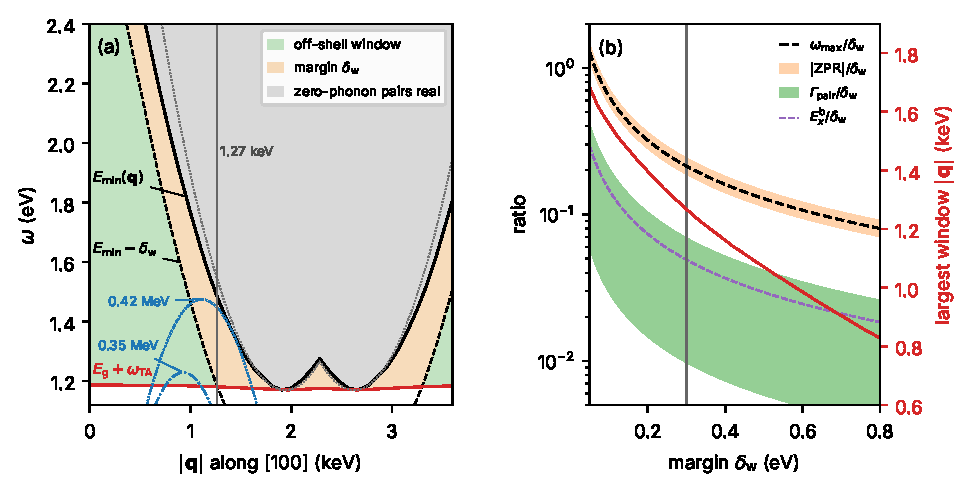
\includegraphics[width=\linewidth]{figures/ch13/fig13_6.pdf}
  \caption{The off-shell window of silicon. (a)~The plane of momentum transfer $|\vect{q}|$ along [100], the valley axis, and energy deposited $\omega$. Black: the zero-phonon edge $E_{\mathrm{min}}(\vect{q})$ from the PBE bands of \cref{fig:3-si-bands} on a $48^3$ grid, with the conduction bands shifted to the measured gap of \SI{1.17}{eV} (dotted: the parabolic valley, pair mass $1.19\,m_e$); dashed: $E_{\mathrm{min}} - \delta_{\mathrm{w}}$ with $\delta_{\mathrm{w}} = \SI{0.3}{eV}$; red: the phonon-assisted onset $\Eg + \omega_{\mathrm{TA}}(\vect{Q}^*)$ of \cref{eq:13.1-EPA}, with the PBE force constants of \cref{sec:5.2} and $\vect{Q}^*$ measured to the nearest valley, the Umklapp image of the opposite valley at \SI{2.63}{keV} included. Green: the off-shell window, where the phonon-assisted rate is a channel of its own; orange: the margin, where it is finite but its corrections grow; gray: zero-phonon pairs are real and the Dyson convention of \cref{sec:8.6} applies. Blue: the largest energy deposited by dark matter of 0.35 and \SI{0.42}{MeV}. (b)~The ratios that control the window, against the margin $\delta_{\mathrm{w}}$: top of the phonon band (\SI{64.1}{meV}), zero-point renormalization of the gap (56 to \SI{73}{meV}), width of the pair at the zero-phonon edge for $0.4 \le |\vect{q}| \le \SI{1.4}{keV}$ (3 to \SI{21}{meV}, a deformation-potential estimate with computed constants~\cite{li2021deformation}), and exciton binding energy (\SI{14.7}{meV}). Red, right axis: the largest $|\vect{q}|$ below the valley at which the window is not empty. The vertical line marks $\delta_{\mathrm{w}} = \SI{0.3}{eV}$.}
  \label{fig:13-offshell}
\end{figure}

\Cref{fig:13-offshell}(a) shows the window in the plane of $|\vect{q}|$ and $\omega$. It is a region of that plane, not an interval of $\omega$: at each $\vect{q}$ it runs from the onset $E^{\mathrm{PA}}_{\mathrm{min}}(\vect{q})$ of \cref{eq:13.1-EPA} up to $E^{\mathrm{ren}}_{\mathrm{min}}(\vect{q},T) - \delta_{\mathrm{w}}$, and it is empty where the two meet. At $|\vect{q}| = \SI{1.0}{keV}$ it spans 1.184 to \SI{1.467}{eV}. Along the valley axis it closes at $|\vect{q}| = \SI{1.27}{keV}$ with the computed bands, \SI{1.33}{keV} with the parabolic valley of \cref{sec:13.3}, and it reopens on the far side of the Umklapp image of the opposite valley, beyond \SI{3.30}{keV}. Dark matter just above the onset mass reaches only the bottom of the window. At \SI{0.42}{MeV}, where the zero-phonon line opens along this axis (\cref{sec:13.1}), the largest deposits already lie in the margin.

Between $E^{\mathrm{ren}}_{\mathrm{min}} - \delta_{\mathrm{w}}$ and $E^{\mathrm{ren}}_{\mathrm{min}}$ the amplitude is still finite, but its corrections grow as $1/(E^{\mathrm{ren}}_{\mathrm{min}} - \omega)$ and reach order one at the edge. Above the edge, within a few widths of it, no test function is smooth on the scale of the detuning, and the Dyson split of \cref{sec:8.6} has no meaning. The margin and this shell form the edge band. There we quote only totals, computed from the unexpanded amplitude \cref{eq:8.6-amp}, and no phonon-assisted rate of its own; in particular the onset exponents of \cref{eq:13.3-pon} hold only where the onset lies inside the window (\cref{sec:13.3}).

In a calculation the window is applied point by point. For each bin of $(|\vect{q}|,\hat{\vect{q}})$ the edge is the minimum of the renormalized pair energies on the full grid of $\vect{k}$, not along a symmetry line, and the bins in $\omega$ stop at that edge minus $\delta_{\mathrm{w}}$. The resonant denominators, path A with $p$ empty and path C with $p$ filled, are written as zero-phonon detunings, $\omega - E_{pv}(\vect{k},\vect{q})$ and $E_{cp}(\vect{k}+\vect{Q},\vect{q}) - \omega$, so that their smallness inside the window is visible and the energies in them are the ones that define the edge. Any smearing of the energy delta function must be small compared with $\delta_{\mathrm{w}}$, or it leaks the zero-phonon continuum into the window.

\subsection{Resonant denominators beyond the window}

Above $E^{\mathrm{ren}}_{\mathrm{min}}(\vect{q},T)$ a resonant intermediate state is a real pair. In path A it is the pair $m = (p,\vect{k}+\vect{q};\,v,\vect{k})$ with an electron in an empty band, which then emits or absorbs the phonon. In path C it is $m = (c,\vect{k}';\,p,\vect{k}+\vect{Q})$ with a hole in a filled band, which relaxes into $(v,\vect{k})$ by the phonon. Near such a state we split the amplitude into the resonant term and the rest. The resonant denominator receives the width of the pair, \cref{eq:2.4-width}:
\begin{equation}
  M^\pm_{cv\nu} = \frac{g_{fm}\,\rho_m}{\omega - \tilde E_m + \ii\varGamma_m/2} + g_{fm}\,\mathcal{A}^{\mathrm{off}}_f ,
  \label{eq:13.6-res}
\end{equation}
with $\rho_m = \rho_{pv}(\vect{k},\vect{q})$ and $g_{fm} = g_{cp\nu}(\vect{k}+\vect{q},\vect{Q})$ for path A, $\rho_m = \rho_{cp}(\vect{k}+\vect{Q},\vect{q})$ and $g_{fm} = g_{pv\nu}(\vect{k},\vect{Q})$ for path C, $\tilde E_m$ and $\varGamma_m$ the renormalized energy and the width of the pair, and $g_{fm}\mathcal{A}^{\mathrm{off}}_f$ the sum of all other terms of \cref{eq:13.2-M}; the minus sign of path C in \cref{eq:13.2-paths} is absorbed into $\rho_mg_{fm}$. A path C term has to be taken from the four-path form \cref{eq:13.2-paths}, with its many-body denominator, before the band-sum theorem is used: the width belongs to the propagator of the real pair $m$, and the theorem holds only on the energy shell (\cref{sec:13.2}). This is the amplitude \cref{eq:8.6-amp} of the level-and-band model with $\Upsilon_m$ dropped, a correction of order $g^2$.

Squared, \cref{eq:13.6-res} contains the Lorentzian $|g_{fm}\rho_m|^2/[(\omega - \tilde E_m)^2 + \varGamma_m^2/4]$, which \cref{eq:2.4-split} splits into $(2\pi/\varGamma_m)\delta(\omega - \tilde E_m)$, the finite part $\operatorname{fp}(\omega - \tilde E_m)^{-2}$ and a correction of relative order $\varGamma_m^2/\delta_{\mathrm{F}}^2$. Summed over the final states of the phonon, the delta term is $|\rho_m|^2\delta(\omega - \tilde E_m)$ times $\sum_f2\pi|g_{fm}|^2\delta(E_f - \tilde E_m)/\varGamma_m$, the fraction of the decays of $m$ that go into phonon emission. It is the zero-phonon pair, created as a real state, followed by its first decay: the cascade of \cref{sec:2.4}. The Dyson convention \cref{eq:8.6-dyson} assigns it to the zero-phonon sector with its residue, and assigns the finite part, the principal-value cross term with $\mathcal{A}^{\mathrm{off}}_f$ and $|\mathcal{A}^{\mathrm{off}}_f|^2$ to the phonon-dressed one. Outside the window, then, the phonon-assisted structure factor is $S^+$ of \cref{eq:8.6-dyson} with the substitutions above, summed over the resonances of both paths, and the zero-phonon one is $S^0$ with renormalized pairs. The two add up to the response to order $g^4$ and $\varGamma_m^2/\delta_{\mathrm{F}}^2$, against any test function smooth on the scale of the detuning $\delta_{\mathrm{F}}$ (\cref{sec:8.6}).

A computed phonon-assisted table beyond the window differs from one inside it in three ways: it need not be positive, it must not be mixed with another convention, and it is defined only near narrow lines. The finite part is negative against a narrow test function, so $S^+$ is not a positive spectrum near $\tilde E_m$, and a computed phonon-assisted table may contain negative bins near the edge; only $S^0 + S^+$ is positive. A Lorentzian zero-phonon line added to the resummed square of \cref{eq:13.6-res} counts the cascade twice, an error of order one. Added to the finite part it counts the off-shell weight twice, an error of order $g^2$ (\cref{sec:8.6}). The rate of \cref{sec:13.3} continued past the edge with a small numerical broadening in place of the width produces a delta term weighted by the inverse broadening, a cascade with an arbitrary weight.

The split is well defined only while $\varGamma_m \ll \delta_{\mathrm{F}}$, with $\delta_{\mathrm{F}}$ the distance of $\tilde E_m$ to the nearest structure of the one-phonon continuum: the zero-phonon edge itself, a threshold for emitting a further phonon, or the onset of a new valley or band. In silicon, with the widths of 3 to \SI{21}{meV} estimated above and detunings of a few tenths of an eV away from such structures, $\varGamma_m/\delta_{\mathrm{F}}$ is 0.01 to 0.1, and by \cref{eq:8.6-ambiguity} the zero-phonon weight is fixed to that order. Within a few widths of each structure it is not, and only totals are quoted, as at the edge of the window.

\subsection{The Fano term near a resonance}

When a real pair $m$ decays, the phonon it emits first interferes with the same phonon emitted directly by the off-shell paths, and \cref{eq:8.6-fano} shifts the branching of the first emission by the Fano coefficients $c^{\mathrm{F}}_\nu = \varGamma^{\mathrm{tot}}_m\Imag(\rho_m^*\mathcal{A}^{\mathrm{off}}_\nu)/|\rho_m|^2$. Their size near a resonance follows from \cref{eq:13.6-res}. With $\phi_\nu$ the phase of $\rho_m^*\mathcal{A}^{\mathrm{off}}_\nu$,
\begin{equation}
  |c^{\mathrm{F}}_\nu| = \frac{\varGamma^{\mathrm{tot}}_m}{\delta_{\mathrm{F}}}\;\frac{|\mathcal{A}^{\mathrm{off}}_\nu|\,\delta_{\mathrm{F}}}{|\rho_m|}\;|\sin\phi_\nu| .
  \label{eq:13.6-fano}
\end{equation}
The middle factor compares the off-shell amplitude with the resonant one at the distance $\delta_{\mathrm{F}}$ from the line. Both are second-order amplitudes with denominators of that size, and the factor is of order one. The Fano coefficients are therefore of first order in $\varGamma_m/\delta_{\mathrm{F}}$, the same order as the ambiguity of the Dyson split and as the branching of the cascade itself, and they need the phase $\phi_\nu$ in addition.

Symmetry controls that phase. In a crystal invariant under inversion combined with time reversal, with an even number of electrons, $(\mathsf{P}\mathsf{T})^2 = +1$ on the many-electron states, every amplitude can be made real, $\sin\phi_\nu = 0$, and the Fano term vanishes (\cref{sec:8.6}). Silicon and germanium satisfy the hypothesis at the level of one-body self-energies, with spin--orbit coupling as well: the single-electron Kramers pairs cannot all be chosen real, but the many-electron states with an even number of electrons can. If the attraction of electron and hole splits a degenerate zero-phonon manifold in a basis that is not invariant, only the sum of the coefficients over the branches vanishes. GaAs has no center of inversion, and its antisymmetric crystal potential gives $\phi_\nu$ a nonzero value. We estimate $|c^{\mathrm{F}}_\nu| \lesssim 0.3\,\varGamma_m/\delta_{\mathrm{F}}$ to first order, with the middle factor of \cref{eq:13.6-fano} set to one and $|\sin\phi_\nu| \le 0.3$ assumed for the antisymmetric part of the GaAs potential, and with Fr\"ohlich widths of a few meV just above the conduction minimum and 20 to \SI{60}{meV} higher up, $\varGamma_m/\delta_{\mathrm{F}}$ is 0.01 to 0.2 away from thresholds (\cref{app:E.14}). The Fano coefficients then move a few percent at most of the first emissions from one branch to another. Since their deviations from the mean average to zero over the branches, they change no total and no number of zero-phonon events, only which phonon the cascade starts with, and the distribution of the number of pairs by at most $\max_\nu|c^{\mathrm{F}}_\nu|$. Near each threshold $\delta_{\mathrm{F}}$ falls toward $\varGamma_m$, \cref{eq:13.6-fano} reaches order one and the expansion ends; these shells are excluded and quoted as totals. Inside the window no zero-phonon pair is real, and the Fano term does not exist.
